As for manipulating objects, the architecture is only focused on grasping. The input is the specific target entity in the world model \acrshort{ed}. The output is the grasp motion, i.e. joint positions for all joints in the kinematic chain over time. Figure \ref{fig:grasping_pipeline} shows the grasping pipeline.
\begin{figure}[h]
    \centering
    %\vspace{-0.3cm}
	\includegraphics[width = 1\linewidth]{Figures/grasping_pipeline}
    %\vspace{-1em}
	\caption{Custom grasping pipeline base on ED, MoveIt and a separate grasp point determination and approach vector node.}
	\label{fig:grasping_pipeline}
    %\vspace{-0.5cm}
\end{figure}
A python executive queries the current pose of the entity from \acrshort{ed}. The resulting grasp pose goes to the grasp precompute component which makes sure that the object is approached in a proper way. MoveIt will produce joint trajectories over time with use of the current configuration, the URDF model and the final configuration. Note that MoveIt currently does not take any information from \acrshort{ed} into account. Finally, the trajectories are sent to the reference interpolator which sends the trajectories either to the controllers or the simulated robot.
\\\\
The grasping pipeline is extended with an empty spot designator and grasping point determination. The empty spot designator searches in an area for an empty spot to place an object by using the occupied area by other objects in this area.
\\
The grasp point determination uses the information about the position and shape of the object in \acrshort{ed} to determine the best grasping point. The grasping point is a vector relative to the robot. An example of the determined grasping point is shown in Figure \ref{fig:grasping_point_determination}.
 \begin{figure}[h]
    \centering
    %\vspace{-0.3cm}
	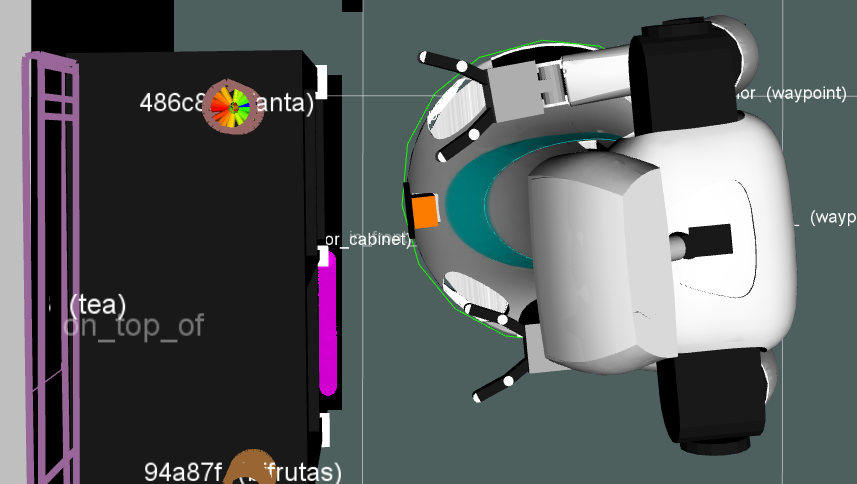
\includegraphics[width = 0.8\linewidth]{Figures/grasp_point_determination}
    %\vspace{-1em}
	\caption{Grasping point determination result for a cylindric object.}
	\label{fig:grasping_point_determination}
    %\vspace{-0.5cm}
\end{figure} 